\chapter{球員設計}
\section{設計概念}
    原先球員設計是一人設計一種球員,但經過討論後,發現如果一人一種機器人會造成整個場面很混亂,所以最後選擇分成兩對,一隊一種球員設計。使用上述方法,觀看者可以更好的分辨隊伍,操作者也能明確地確認隊友。\\[6pt]

\section{球員設計(一)}
    球員一採用縮小本體體積,兩側伸出較長的竿子阻饒敵人搶球,且能更好的控制球。如(圖.\ref{球員})\\[6pt]\\
\begin{figure}[hbt!]
\center
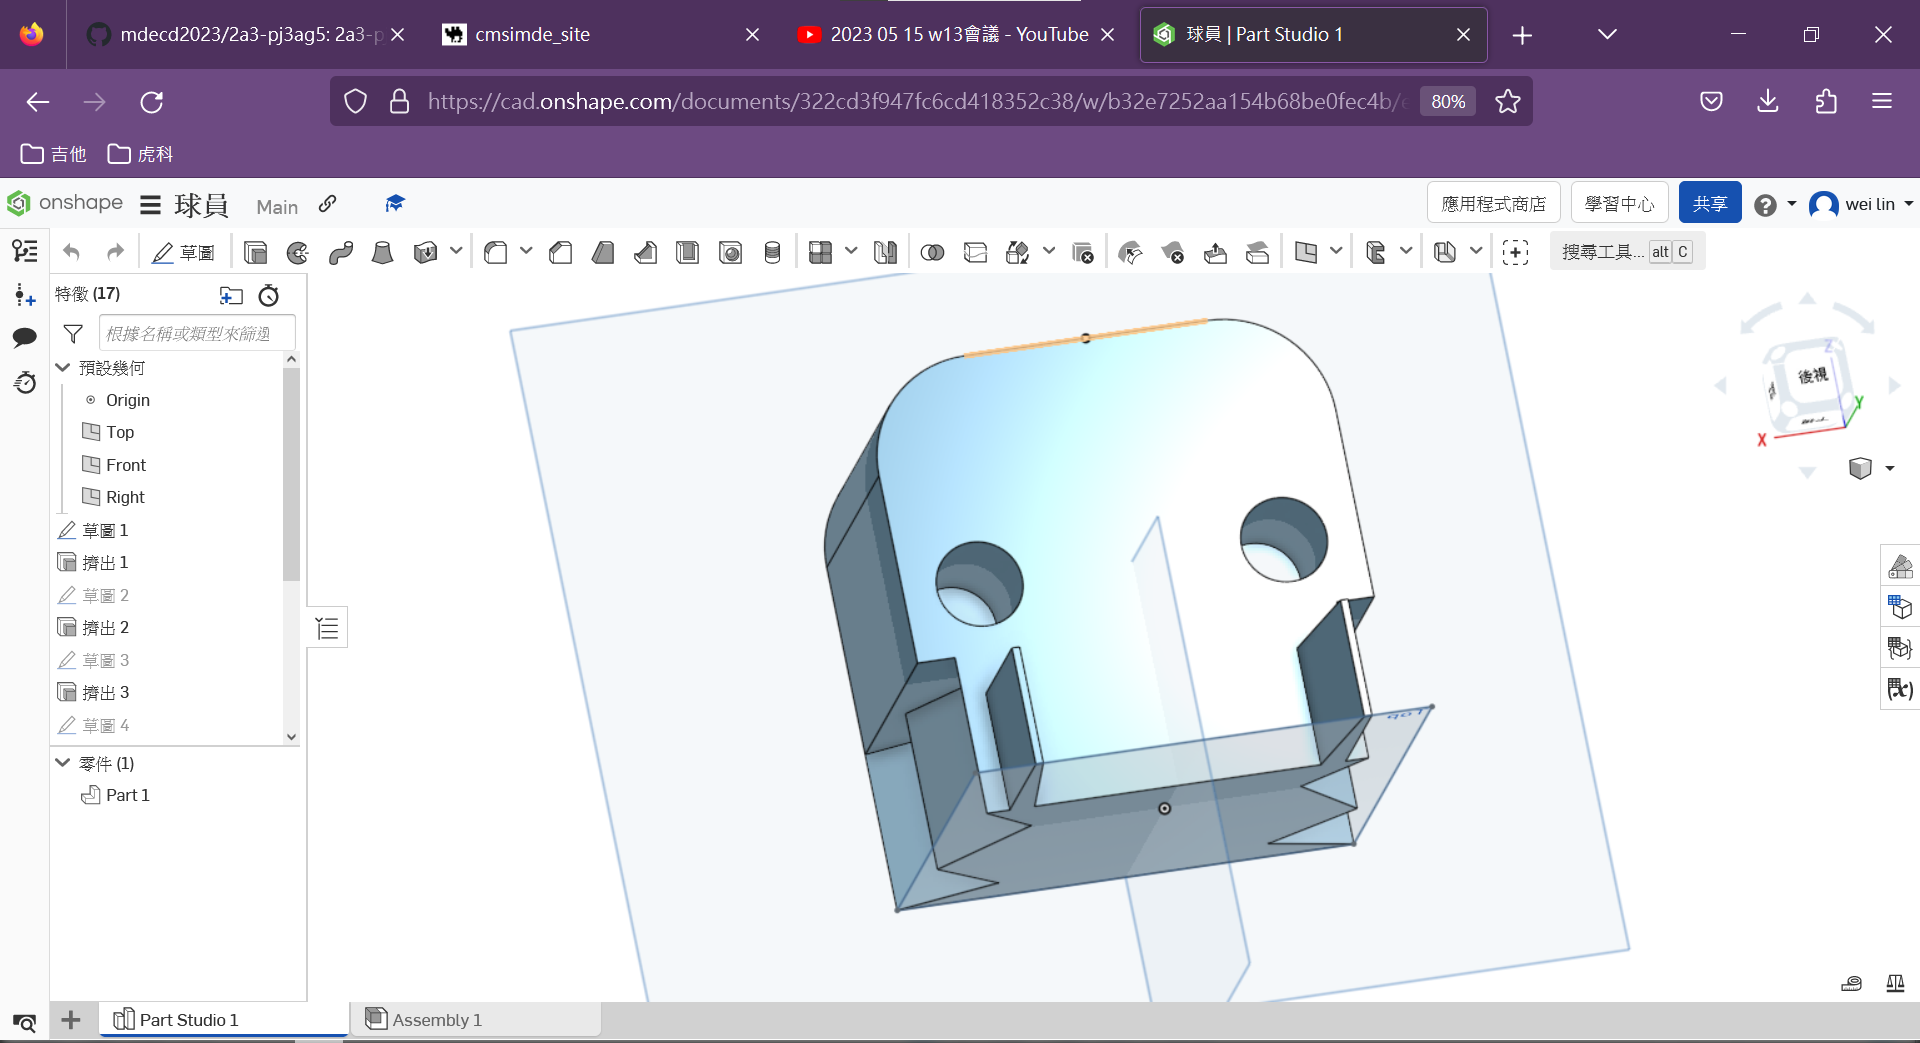
\includegraphics[width=13cm]{球員}
\caption{\Large 球員(一)}
\label{球員}
\end{figure}

\newpage
\section{球員設計(二)}
    球員二體型相對於球員一,是比較大,但有較大的範圍可以搶足球,兩隻手臂前端稍微向內延伸,為了讓足球進入手臂後不容易再滾出,而去做的設計。如(圖.\ref{車車2})所示。\\[6pt]\\
\begin{figure}[hbt!]
\center
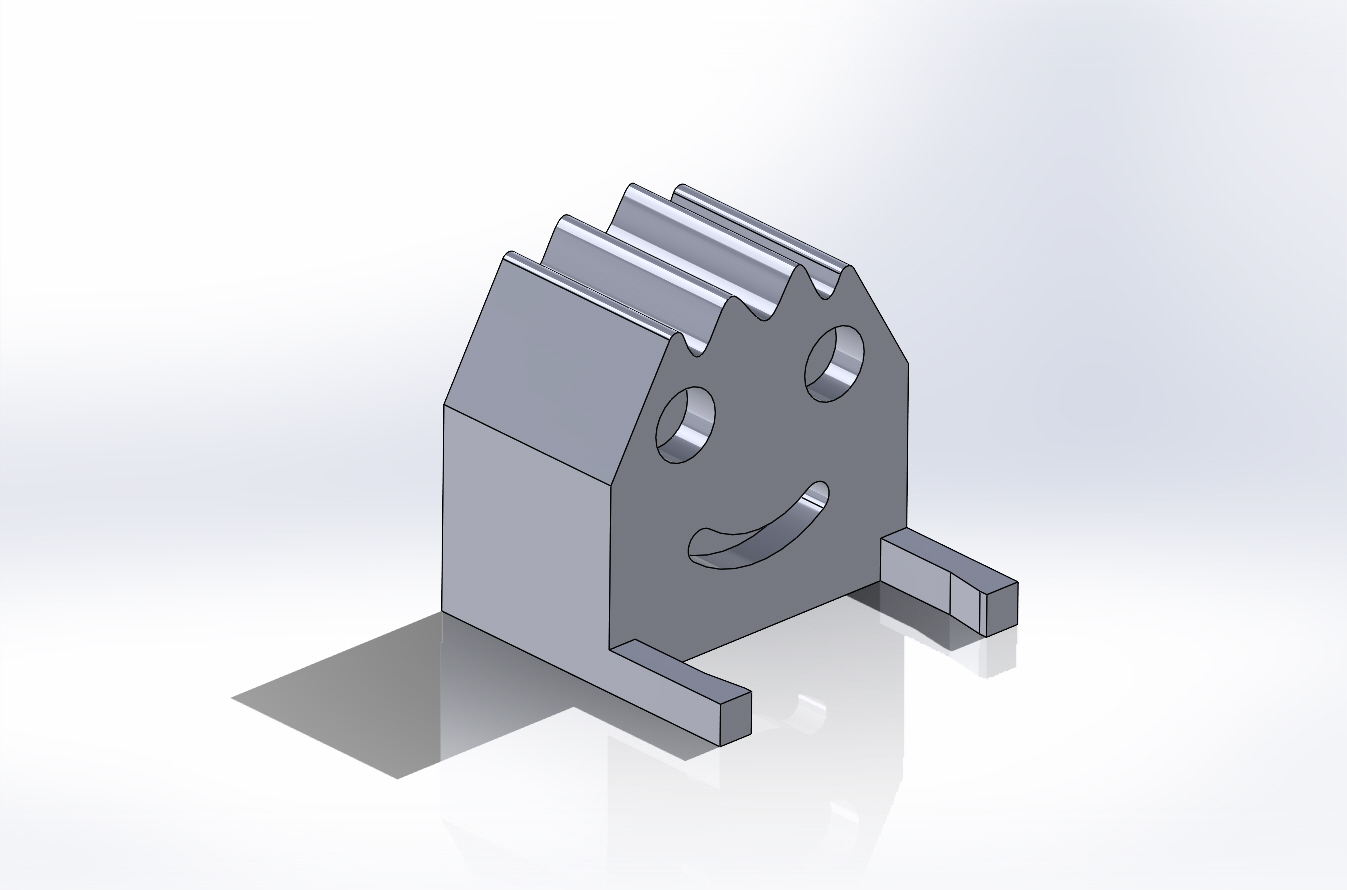
\includegraphics[width=13cm]{車車2}
\caption{\Large 球員(二)}
\label{車車2}
\end{figure}